\documentclass[11pt]{article}
\usepackage[utf8]{inputenc}
\usepackage[french]{babel}
\usepackage[T1]{fontenc}
\usepackage{verbatim}
\usepackage{graphicx}
\usepackage{fullpage}
\usepackage{hyperref}
\usepackage[usenames,dvipsnames]{color}
\usepackage{textcomp}
\usepackage{fix-cm}
\usepackage{float}
\usepackage{biblatex}
\usepackage{setspace}
\author{Contzen Laurent}
\bibliography{asi.bib}
\onehalfspacing
\begin{document}

\begin{titlepage}  
  \begin{flushleft}
    Contzen Laurent
  \end{flushleft}
  \begin{center}
    \vspace{80mm}\LARGE{\textbf{STIC-B-415 : Architecture des Systèmes d'Information.} \\    
      Les bases de données de type NoSQL.}
  \end{center}
  \begin{flushright}
    \vspace{90mm}
    Année Académique 2011-2012.             
  \end{flushright}
\end{titlepage}

\vspace*{\fill}
\begin{flushright}
  A DBA walks into a bar and leaves immediatly. \\
  He couldn't find a table. \\
  \textit{- Anonymous}
\end{flushright}
\vspace*{\fill}
\newpage
\tableofcontents
\newpage
\listoffigures
\newpage

%% \begin{spacing}{1.5}
\section{Introduction}
Opposées \colorbox{BrickRed}{\textbf{FIXME}} aux bases de données relationnelles, les bases de données faisant partie de la mouvance NoSQL sont non relationnelles, distribuées, horizontalement scalable (\colorbox{BrickRed}{\textbf{FIXME}}) et open-source. Bien que le terme NoSQL ait été utilisé pour la première fois en 1998 par Carlo Strozzi pour nommer le système de gestion de bases de données (SGDB) relationnel qu'il venait de développer, la vraie naissance de cette mouvance eut lieu en 2009 lorsque Eric Evans, un employé de la société Rackspace, utilisa ce terme dans une discussion sur les bases de données distribuées. Ces dernières devenant de plus en plus importantes dans le web actuel, il était logique de travailler sur le sujet quitte à remettre en question un modèle en place depuis plusieurs décennies. Il est important de souligner que le terme NoSQL est généralement interprété comme ``Not only SQL'' et non comme ``No SQL''. En effet, certains SGDB de la famille NoSQL utilisent une partie des concepts fondamentaux au modèle relationnel.
\section{Historique}
Les bases de données ont toujours été quelque chose de fondamental en informatique. En effet, stocker de grandes quantité d'informations et pouvoir y accéder et les traiter rapidement et efficacement est un des buts fondamentaux de cette discipline.

Au départ, chaque système était lié à son propre SGDB, étudié et optimisé pour lui. Ceci posait évidemment, comme beaucoup de choses à cette époque, de gros problèmes de portabilité de données et changer un système informatique avait d'énormes implications. Il était donc nécessaire et urgent de standardiser ça, ce qui fut fait par le Database Task Group qui proposa en 1971 un standard qui fut connu en tant que Codasyl Approach. Cette approche était navigationnelle et basée sur une navigation manuelle d'un ensemble d'informations disposées en ``réseau''. Bien que cela puisse paraître parfaitement inefficace de nos jours, une telle approche représentait déjà un grand gain de performances à l'époque.

C'est un peu plus tard dans cette même décennie qu'un ingénieur travaillant chez IBM, Edgar Codd, révolutionna le monde des bases de données avec son article ``A Relational Model of Data for Large Shared Data Banks'' qui posa les fondations des bases de données relationnelles. Les principes énoncés dans cet articles furent rapidement implémentés et testés, et un langage de requêtes standardisé, le SQL\footnote{Structured Query Language}, fit son apparition en même temps. Les bases de données relationnelles utilisant SQL se sont très vite répandues et plusieurs implémentations telles que DB2, Microsoft SQL Server, PostgreSQL ou encore MySQL apparurent et s'imposèrent comme un standard de facto.

Ce n'est que bien plus tard, à la fin des années 2000, que ce modèle fut largement remis en question et plusieurs modèles de bases de données non relationnelles firent alors leur apparation.

\section{Le modèle relationnel}
Pour pouvoir comprendre les différences entre le modèle relationnel et la mouvance NoSQL, commençons par brièvement décrire ce modèle historique avant d'en montrer un bref exemple et d'analyser ses avantages et inconvénients.
\subsection{Description}
Dans une base de données relationnelle, les données sont organisées sous forme de tables dans lesquelles les colonnes sont les champs et le contenu des lignes les données. Une ligne d'une table est donc un ensemble de données représentant les valeurs des différents champs pour une même entité. Le modèle entité-association est utilisé afin de décrire les entités (les champs qui les composent, la clé primaire unique, etc) et les relations entre elles. Un schéma décrivant l'application de ce modèle aux données allant être traitées ainsi que les contraintes les concernant doit être établi à l'avance et ne peut être changé que en recréant les tables.

Le langage SQL sera ensuite utilisé afin d'effectuer des transactions dans la base de données, une transaction étant une action telle qu'insérer une nouvelle entrée dans une table, mettre à jour un champ ou extraire des informations. SQL offre plusieurs types de transactions pouvant être combinées telles que la sélection, la jointure (sélection d'éléments à partir d'informations contenues dans différentes tables), le produit cartésien et bien d'autres. 
\subsection{Exemple}
Imaginons une table Persons contenant des informations sur des personnes et établissons que les champs nécéssaires à la description d'une personne soient son identificateur unique (un nombre différent pour chacun), sa ville de naissance et son année de naissance. Un telle table pourrait être :
\begin{figure}[H]
  \centering
  \begin{center}
    \begin{tabular}{| c | l | l | l | l |}
      \hline
      \textbf{\underline{Id}} & \textbf{Name} & \textbf{PlaceOfBirth} & \textbf{YearOfBirth} \\
      \hline
      \hline
      1 & David Robert Jones & Brixton & 1947 \\
      \hline
      2 & Oliver Dene Jones & London & 1986  \\
      \hline
      3 & Kathleen Brien & London & 1989 \\
      \hline
      4 & Peter Tong & Dartford & 1960 \\
      \hline
      5 & Annie MacManus & Dublin & 1978 \\
      \hline
      \vdots & \vdots & \vdots & \vdots \\
      %\hline
    \end{tabular}
  \end{center} 
  \caption{Exemple de table dans une base de données relationnelle.}
\end{figure}
Par souci de concision pour cet exemple nous nous limiterons à cette table et ommettrons d'en définir d'autres ainsi que de définir le schéma entité-association.

La requête effectuée afin d'extraire l'entièreté des informations de la table Persons pourra être : \\
\verb|SELECT * FROM Persons;| \\
Il est possible de sélectionner uniquement les personnes nées à Londres : \\
\verb|SELECT * FROM Persons WHERE PlaceOfBirth=``London'';| \\
La requête suivante permet d'obtenir le nom des personnes nées à Brixton en 1947 : \\
\verb|SELECT Name FROM Persons WHERE PlaceOfBirth=''Brixton'' AND YearOfBirth=''1947'';|
\subsection{Avantages et inconvénients}
Le modèle relationnel repose sur des fondements mathématiques théoriques tels que l'algèbre relationnelle et le calcul relationnel tuple, ce qui implique que ce modèle est extrêmement formalisé et demande beaucoup de rigueur. Ce formalisme apporte des garanties sur la fiabilité d'un système en production mais requiert une grande réflexion sur la structure de la base de données avant de commencer à l'implémenter et l'utiliser. Ceci peut s'avérer être très problématique dans le cadre du web actuel dans lequel il est parfois extrêmement difficile de pouvoir prévoir à l'avance les besoins d'une application et la migration d'un schéma à un autre dans une base de données fort peuplée est une opération très délicate pouvant s'avérer très coûteuse.

Cette même évolution du web oblige les SGBD à faire face à d'autres défis que le modèle relationnel ne sait pas relever, ou que difficilement. Il est utile, voire nécéssaire, de pouvoir redimmensionner facilement et à la volée les moyens techniques soutenant les bases de données (nombre de serveurs utilisés par exemple) ainsi que d'avoir la possibilité de distribuer les bases de données dans divers data centers à travers le monde. Pouvoir changer la structure de la base de données pour offrir de nouvelles fonctionnalités à l'utilisateur tout en offrant une continuité de service est tout aussi primordial.

\section{ACID et CAP}
Les deux mouvances de systèmes de gestion de bases de données nous occupant ici sont basées sur des ensembles de principes de base différents connus sous les acronymes ACID (modèle relationnel) et CAP (mouvance NoSQL). Il est toutefois à noter que certains SGBD de la famille NoSQL tels que Neo4j (présenté section \ref{neo4j}) respectent ACID.
\subsection{ACID}
ACID est l'acronyme de \textbf{A}tomicity, \textbf{C}onsistency, \textbf{I}solation and \textbf{D}urability. L'atomicité garantit qu'une transaction est soit une réussite, soit un échec, sans statut intermédiaire. Ceci implique que si une transaction échoue l'entièreté des modifications qu'elle apportait devra être annulée. Par exemple, il sera impossible qu'une insertion échoue mais qu'une partie des données la composant (\colorbox{BrickRed}{\textbf{FIXME}}) soient tout de même présentes dans la base de données. \\
Le principe de consistance signifie que la base de données est dans un état correct avant et après chaque transaction. L'atomicité et la consistance sont donc deux principes intimement liés. \\
L'isolation va quand à elle forcer les transaction à être indépendantes les unes des autres. Si deux transactions doivent modifier une même donnée l'une des deux sera mise en attente jusqu'à ce que la première aie fini. \\
Enfin, la durabilité implique qu'une fois qu'une transaction est terminée et réussie les modifications qu'elle a apporté resteront dans la base de données, même dans le cas où le système tombe en panne \colorbox{BrickRed}{\textbf{FIXME}}.

Cet ensemble de principes assure donc que la base de données restera cohérente dans tous les cas et permet d'éviter au maximum la corruption ou perte de données. Mais tout ceci a un coût. Par exemple, si la base de données doit subir une très grande quantité de transactions en très peu de temps le principe d'isolation va fortement ralentir le processus. Ceci peut s'avérer très problématique dans le cadre des réseaux sociaux : le nombre de messages à la seconde sur Twitter lors de gros évènements, par exemple, peut vite atteindre un niveau trop élevé pour qu'une base de données respectant le principe d'isolation puisse absorber la charge. \colorbox{BrickRed}{\textbf{FIXME}}
\subsection{CAP}
Le théorème CAP, aussi connu sous le nom de Brewer's theorem (du nom d'Eric Brewer qui l'a proposé en 2000 lors d'un symposium sur l'informatique distribuée), statue qu'il est impossible pour tout système de données partagées de garantir simultanément les trois principes suivants : consistance (\textbf{C}onsistency), disponibilité (\textbf{A}vailability) et tolérance à la partition (\textbf{P}artition tolerance). Ce théorème a été prouvé en 2002 par Seth Gilbert et Nancy Lynch du MIT\cite{cap}. \\
Le principe de consistance dans CAP est à interpréter totalement différemment de la manière énoncée pour ACID : il représente dans le cas présent le fait que lorsqu'une donnée est insérée ou modifiée toute personne y accédant aura toujours la dernière version de l'information. \\
La disponibilité, quant à elle, signifie qu'il est possible de considérer que toute requête envoyée à la base de données recevra une réponse sur son succès ou son échec. Pour arriver à cet objectif les bases de données seront répandues sur énormément de serveurs physiques agissant comme une seule base de données avec la puissance de tous les serveurs la composant. \\
Pour finir, la tolérance à la partition implique que l'ensemble des données sera toujours accessible, même si une partie des serveurs est totalement inaccessible. Ceci va permettre de diviser la base de données entre plusieurs data centers et les données seront répliquées à différents endroits mais pas dans l'entièreté des data centers. Si une information doit être écrite dans un noeud A temporairement inaccessible, elle sera écrite dans un autre noeud qui la lui transmettra lorsqu'il sera à nouveau fonctionnel. 
\subsection{Cas d'utilisation}
%Comme le démontre la différence entre CAP et ACID, les bases de données relationnelles et les bases de données de type NoSQL ne suivent pas les mêmes idées et vont avoir des cas d'utilisation différents. 
ACID et CAP étant fort différents, les bases de données respectant l'un ou l'autre auront des cas d'utilisation différents. Tout ce qui a un rapport avec le système bancaire, par exemple, devra avoir la certitude que les données sont consistantes (au sens ACID du terme) et qu'aucune donnée ne sera jamais perdue. On peut aussi considérer que les changements de structures de bases de données dans ce domaine sont assez rares, et qu'il n'y a pas de pics d'utilisation rares et d'intensité sans commune mesure avec l'utilisation normale nécéssitant une grande élasticité au niveau de l'offre de ressources. Les bases de données NoSQL suivant CAP ne sont donc absolument pas adaptées à ce type de domaine. %Les bases de données NoSQL ne sont donc absolument pas adaptées, actuellement, à ce type de domaine.

Par contre, les réseaux sociaux sont un excellent exemple de situations dans lesquelles les bases de données respectant CAP sont bien plus adaptées que celles suivant le modèle historique ACID. En effet, la quantité de données circulant dessus est astronomique (et en constante expansion) mais très irrégulière, et un délai dans la mise à jour des informations des utilisateurs (le temps de répliquer l'information à travers les data centers concernés) n'aura aucune conséquence grave. De plus, la scalability (\colorbox{BrickRed}{\textbf{FIXME}}) des serveurs est quelque chose de crucial. Avoir en permanence des serveurs capables de tenir les pics de charge les plus rares coûterait une fortune et ces serveurs seraient presque tout le temps largement sous utilisés. Pouvoir modifier la capacité du système pour absorber un pic et puis revenir à la situation normale permet donc d'effectuer de grandes économies sans lesquelles certaines entreprises ne pourraient pas survivre. Par exemple, les MTV Video Music Awards ont engendré 8868 tweets par seconde sur Twitter le 28 août 2011\cite{tweetspersecond}, alors qu'en temps normal le nombre de tweets par seconde est largement inférieur à cela. Devoir maintenir des serveurs pouvant résister à cette charge en permanence signifierait probablement la faillite de l'entreprise Twitter.

Il existe beaucoup d'applications utilisant des systèmes relationnels et NoSQL en coopération, chacun pour des tâches différentes. Par exemple, le site \url{reddit.com}, site communautaire de ``social bookmarking'' classé 114\up{ème} mondial au classement Alexa des sites ayant le plus de traffic\footnote{\url{http://www.alexa.com/siteinfo/reddit.com}}, utilise en parallèle les SGBD PostgreSQL et Apacha Cassandra.

\section{Les différents types de SGBD NoSQL}
La mouvance NoSQL est composée d'un ensemble de systèmes de gestion de bases de données partageant donc un esprit commun et un ensemble de buts à atteindre mais les techniques d'implémentation varient beaucoup de l'un à l'autre. Il est toutefois possible d'identifier plusieurs grandes familles partageant aussi l'aspect technique du type d'implémentation. 
%% \begin{center}
%%   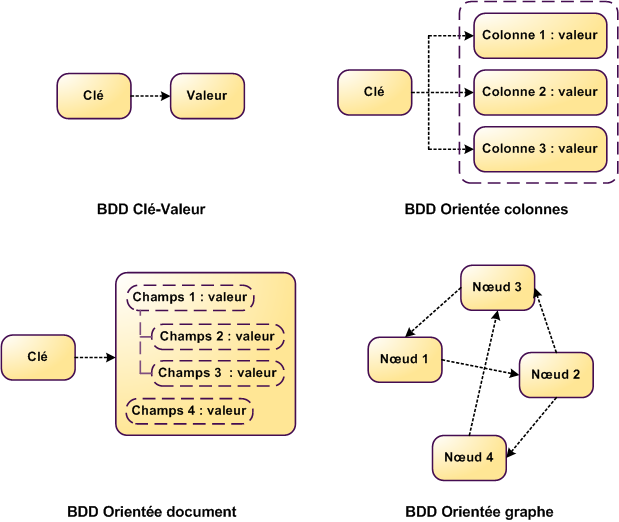
\includegraphics[width=12cm]{nosql.png}
%% \end{center}
\subsection{Les bases de données de type Key-Value}
%\subsubsection*{Description}
\begin{figure}[H]
  \centering
  \begin{center}
    \includegraphics[width=6cm]{keyvalue2.png}
  \end{center}
  \caption{Modèle Key-Value\cite{tourhorizon}}
\end{figure}
Les bases de données de type Key-Value (clé-valeur) peuvent être vues comme de très grandes tables de hachage. L'idée de base repose sur le fait que dans certaines applications la plupart des accès à la base de données ne sont que des lectures ou écriture à partir d'un identifiant. Dans ce cas, il n'est pas nécessaire d'avoir toute la puissance du SQL et, surtout, de devoir subir la lourdeur qui y est associée puisque la plupart des possibilités du SQL ne seront jamais utilisées. Dans ce modèle, la base de données considère la valeur comme un bloc binaire sans savoir ce qu'il contient et ne sais donc faire aucune opération dessus si cela s'avérait nécessaire.

Techniquement, les données seront insérées dans une table partitionnée utilisant un mécanisme de hachage consistant, ce qui permet de répartir uniformément la charge et la quantité de données entre les différentes tables. Ces données seront ensuite répliquées sur d'autres serveurs pouvant contenir chacun plusieurs partitions afin de limiter le nombre minimum d'instances de réplication nécessaires. Il reste alors la consistance à garantir. Pour avoir une consistance parfaite, il serait nécessaire de s'assurer que chaque changement dans une table est bien répliqué dans toutes les instances contenant cette partition mais ceci a évidement un coût niveau efficacité. On va alors définir un taux de consistance souhaité, et s'assurer que au minimum ce pourcentage là des instances est mis à jour. Un mécanisme similaire sera mis en place pour assurer la consistance lors des écritures. Ceci permet de perdre un peu de la certitude de la consistance des données mais d'optimiser l'efficacité du service.
%\subsubsection*{Redis} 
\begin{figure}[H]
  \centering
  \begin{tabular}{l | l}
    \textbf{Nom} & Redis \\
    \textbf{Créateur} & Salvatore Sanfilippo \\
    \textbf{Apparition} & 2009 \\
    \textbf{Financement} & Sponsorisé par VMware \\
    \textbf{Licence} & BSD \\
    \textbf{Ecrit en} & C \\
    \textbf{Bindings en} & ActionScript, C, C++, C\#, Clojure, Common Lisp, Erlang, Fancy, \\
    &  Go, Haskell, haXe, Io, Java, Lua, Node.js, Objective-C, Perl, PHP, \\
    & Pure Data, Python, Ruby, Scala, Smalltalk, Tcl\\
    \textbf{Exemple d'utilisation} & Craiglist \\
    \textbf{Informations} & \url{http://redis.io/}
  \end{tabular}
  \caption{Présentation de Redis, SGBD Key-Value}
\end{figure}
\subsection{Les bases de données orientées document}
%\subsubsection*{Description}
\begin{figure}[H]
  \centering
  \begin{center}
    \includegraphics[width=6cm]{document2.png}
  \end{center}
  \caption{Modèle orienté document\cite{tourhorizon}}
\end{figure}
Cette famille de SGBDs est une extension du modèle Key-Value. La conception de ce modèle est partie de l'observation du  fait que les pages web renseignent souvent un ensemble d'informations ayant un lien clair (par exemple un même utilisateur) mais qui devraient être stockées dans beaucoup de tables différentes dans une structure relationnelle, ce qui serait très coûteux en jointures logiques. Une base de données orientée documents disposera, à l'instar du modèle key-value, d'une clé pour accéder aux données mais ces dernières seront ici enregistrée sous forme de  document structuré (type document XML) dont le SGDB aura connaissance du contenu. Cette connaissance des données permettra d'effectuer des opérations dessus, sans toutefois avoir toutes les possibilités (et à nouveau la lourdeur) du SQL. \colorbox{BrickRed}{\textbf{FIXME}}

L'implémentation d'une base de données orientée document sera sensiblement la même que celle d'une base de données de type key-value mais il lui sera rajouté la ``conscience'' des données qu'elle contient ainsi que des mécanismes de traitements spécifiques à ces données : requêtes plus élaborées, accès à une partie des données associées à une clé sans devoir en charger l'entièreté, modifications de certains champs seulement, etc. C'est donc en quelque sorte un mélange entre les philosophies SQL et NoSQL.

Cette famille, dont le but est de prendre le meilleur des deux mouvances, permettra par exemple de stocker une grande quantité d'informations qui aurait été plus limitée dans le modèle relationnel parfois trop rigide.
%\subsubsection*{CouchDB et MongoDB}
\begin{figure}[H]
  \centering
  \begin{tabular}{l | l | l}
    \textbf{Nom} & CouchDB & MongoDB \\
    \textbf{Créateur} & Damien Katz & 10gen \\
    \textbf{Apparition} & 2005 &  2009 \\
    \textbf{Financement} & Couchbase, Cloudant & 10gen \\
    \textbf{Licence} & Apache 2.0 & GNU Affero GPL\\
    \textbf{Ecrit en} & Erlang & C++\\
    \textbf{Bindings en} & Javascript, .Net, Java, & C, C++, Erlang, Haskell, \\
    & Scala, Perl, PHP, Ruby, Python, & Java, Javascript, .NET, Perl,\\
    & Common Lisp, Clojure, Lua &  PHP, Python, Ruby, Scala \\
    \textbf{Exemple d'utilisation} & Apple, BBC, CERN & FourSquare, Github \\
    \textbf{Informations} & \url{http://couchdb.apache.org/} & \url{http://www.mongodb.org/}
  \end{tabular}
  \caption{Présentation de CouchDB et MongoDB, SGBD orientés document}
\end{figure}
\subsection{Les bases de données orientées colonnes}
%\subsubsection*{Description}
\begin{figure}[H]
  \centering
  \begin{center}
    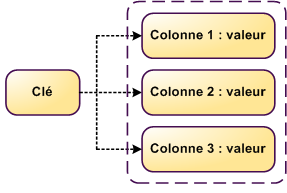
\includegraphics[width=6cm]{columns.png}
  \end{center}
  \caption{Modèle orienté colonnes\cite{tourhorizon}}
\end{figure}
Les bases de données orientées colonnes sont elles aussi une extension du type key-value et un mélange avec des principes du modèle relationnel mais la clé donne ici accès à un ensemble d'informations structurées en colonnes contenant les informations. Les données sont donc structurées mais cette structure présente des avantages non négligeables par rapport aux RDBMSs classiques lorsque la base de données contient énormément d'informations.
\begin{figure}[H]
  \centering
  \begin{center}
    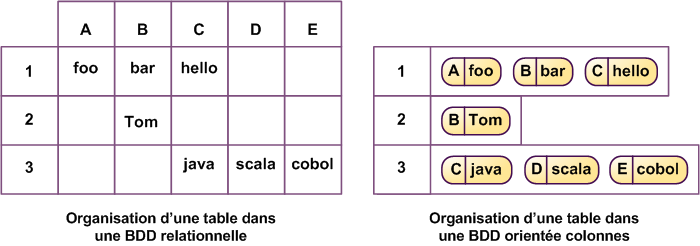
\includegraphics[width=12cm]{nosql-colonnes.png}
  \end{center}
  \caption{Modèle orienté colonnes : différence d'utilisation mémoire\cite{tourhorizon}}
\end{figure}
Tout d'abord, lorsqu'une colonne ne contient pas d'informations pour une clé, la colonne n'existe simplement pas pour elle, ce qui amène à un gain d'espace disque considérable lorsque la base de données contient (ou plutôt devrait contenir en modèle relationnel) plusieurs millions de colonnes. Ensuite, l'ajout de colonnes se faisant à la volée et uniquement pour les entités concernées, l'adaptation de la structure aux nouveaux besoins ou aux changements de design ou de code est immédiate et ne demande aucun effort particulier. Ce modèle permet aussi de faire des requêtes simples sur les données, bien plus simples que leur équivalent SQL.

Apache Cassandra, une base de données orientées colonnes développée par Facebook, étends encore ce modèle en proposant la possibilité de faire des méta-colonnes, c'est à dire de contenir des colonnes dans des colonnes. Cela permet une meilleure organisation des données, et, surtout, une optimisation des requêtes vu que l'ensemble de colonnes à considérer lors d'une requête n'est qu'un sous-ensemble précis défini à l'avance.
%\subsubsection*{Apache Cassandra}
\begin{figure}[H]
  \centering
  \begin{tabular}{l | l}
    \textbf{Créateurs} & Avinash Lakshman et Prashant Malik \\
    \textbf{Apparition} & 2008 \\
    \textbf{Financement} & Apache Software Foundation \\
    \textbf{Licence} & Apache 2 \\
    \textbf{Ecrit en} & Java \\
    \textbf{Bindings en} & Ruby, Perl, Python, Scala, Java, \\
    &   PHP, Clojure, Grails, C++, C\#\\
    \textbf{Exemple d'utilisation} & Facebook, Reddit, Twitter \\
    \textbf{Informations} & \url{http://cassandra.apache.org/}
  \end{tabular}
  \caption{Présentation de Apache Cassandra, SGBD orienté colonnes}
\end{figure} 
\subsection{Les bases de données orientées graphe}
%\subsubsection*{Description}
\begin{figure}[H]
  \centering
  \begin{center}
    \includegraphics[width=6cm]{graphdb2.png}
  \end{center}
  \caption{Modèle orienté graphe\cite{neo4jwebsite}}
\end{figure}
Les bases de données orientées graphe sont quant à elles en rupture avec les autres catégories de la mouvance NoSQL. En effet, elles sont basées sur la théorie des graphes et ne partagent pas beaucoup de points techniques avec les autres. Les données seront donc organisées en noeuds, arcs et propriétés. 
%% \begin{figure}[H]
%%   \centering
%%   \begin{center}
%%     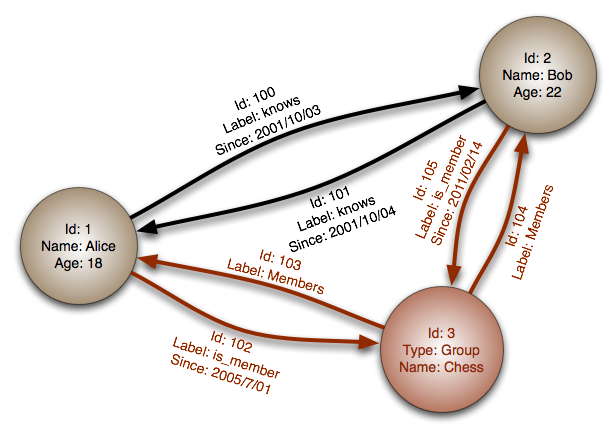
\includegraphics[width=12cm]{nosql_graph.png}
%%   \end{center}
%%   \caption{Modèle orienté graphe : Exemple basique}
%% \end{figure}
Les noeuds, que l'on pourrait comparer à des objets dans la programmation orientée objet, représentent des entités auxquelles sont associées des propriétés et les arcs qui les relient représentent les relations existant entre ces entités et fournissent des informations à leurs propos. Ceci apporte une flexibilité absolue puisqu'il n'y a pas besoin d'établir un schéma de la structure : chaque noeud ou arc peut-être rajouté n'importe quand et contenir n'importe quelle information désirée. Pour les cas où avoir un schéma peut être utile, voire nécessaire, il est tout de même possible d'en définir un qui sera après utilisé pour garantir une cohérence (\colorbox{BrickRed}{\textbf{FIXME}}) entre les noeuds. La théorie des graphes et ses applications étant très utilisée en informatique, il existe déjà des algorithmes très poussés pour le parcours et la recherche par exemple.

Les bases de données orientées graphes permettent d'obtenir certaines opérations extrêmement simplement. Il serait par exemple possible dans un réseau social de calculer le niveau de séparation entre deux personnes en calculant simplement la distance entre les noeuds concernés.

Il est à noter que ce modèle est apparu plusieurs années avant la mouvance NoSQL et certaines de ses implémentations telles que Neo4j respectent ACID. Le point commun entre ce modèle et les autres composant cette mouvance lui permettant d'être considéré comme en faisant partie est son rejet du SQL. \colorbox{BrickRed}{\textbf{FIXME}} 
%\subsubsection*{Neo4j}\label{neo4j}
\begin{figure}[H] \label{neo4j}
  \centering
  \begin{tabular}{l | l}
    \textbf{Créateurs} & Neo Technologies \\
    \textbf{Apparition} & 2003 \\
    \textbf{Financement} & Apache Software Foundation \\
    \textbf{Licence} & GPLv3, AGPLv3, commerciale \\
    \textbf{Ecrit en} & Java \\
    \textbf{Bindings en} & Clojure, Erlang, Gremlin, Groovy, Java, PHP,  \\
    & Python, Ruby, Scala, Grails, Griffon, Qi4j, Roo\\
    \textbf{Exemple d'utilisation} & Box.net, swami.se \\
    \textbf{Informations} & \url{http://neo4j.org/}
  \end{tabular}
  \caption{Présentation de Neo4j, SGBD orienté graphe}
\end{figure}
\section{Conclusion}
La mouvance SQL n'est donc pas un mouvement de rejet en bloc des idées du modèle relationnel. Il s'agit plutôt d'un mouvement d'adaptation du milieu \colorbox{BrickRed}{\textbf{FIXME}} des systèmes de gestion de bases de données aux nouveaux besoins d'applications principalement issues de l'évolution du web. Les concepts de base du modèle relationnel sont remis en question et chaque famille de la mouvance NoSQL va en extraire ce qui lui corresponds le mieux et adapter cette sélection à son esprit.

Le but final de cette mouvance est donc d'offrir un large choix de systèmes de gestion de bases de données pouvant répondre à une grande variété de besoins, et ce tout en retirant les contraintes financières souvent imposées par les RDBMSs \colorbox{BrickRed}{\textbf{FIXME}} 

%% \section*{Sources}
%% \url{http://www.thoughtworks.com/articles/nosql-comparison} \\
%% \url{http://www.linuxjournal.com/article/10770} \\
%% \url{http://nosql-databases.org/} \\
%% \url{http://nosql-database.org/links.html} \\
%% \url{http://en.wikipedia.org/wiki/NoSQL} \\
%% \url{http://en.wikipedia.org/wiki/Dbms} \\
%% \url{http://en.wikipedia.org/wiki/NoSQL_(RDBMS)} \\
%% \url{http://stackoverflow.com/questions/3596461/is-there-any-good-book-on-nosql} \\
%% \url{http://www.computerworld.com/s/article/9135086/No_to_SQL_Anti_database_movement_gains_steam_} \\
%% \url{http://blog.xebia.fr/2010/04/21/nosql-europe-tour-dhorizon-des-bases-de-donnees-nosql/} \\
%% \url{http://www.techrepublic.com/blog/10things/10-things-you-should-know-about-nosql-databases/1772} \\

\newpage
\section{Bibliographie}
\nocite{*}
\printbibliography
%% \end{spacing}
\end{document}

% LocalWords:  Contzen Laurent STIC-B NoSQL SGBDs

% temp :
%% @Comment @Book{engineering2005proceedings,
%%   @Comment  author = {Engineering, International},
%%   @Comment  title = {Proceedings of the 21st International Conference on Data Engineering: 2005},
%%   @Comment  publisher = {IEEE},
%%   @Comment  year = {2005},
%%   @Comment  address = {Piscataway},
%%   @Comment  isbn = {0769522858}
%%   @Comment  }
